
\title{Improving the Robustness of Human Pose Estimation using Fault Estimation on Multi-Modal Data}
\author{Leonardo Benedikt Pohl}
% TITLE
\date{\today}
 
\newlength{\originalVOffset}
\newlength{\originalHOffset}
\setlength{\originalVOffset}{\voffset}   
\setlength{\originalHOffset}{\hoffset}

\setlength{\voffset}{0cm}
\setlength{\hoffset}{0cm}
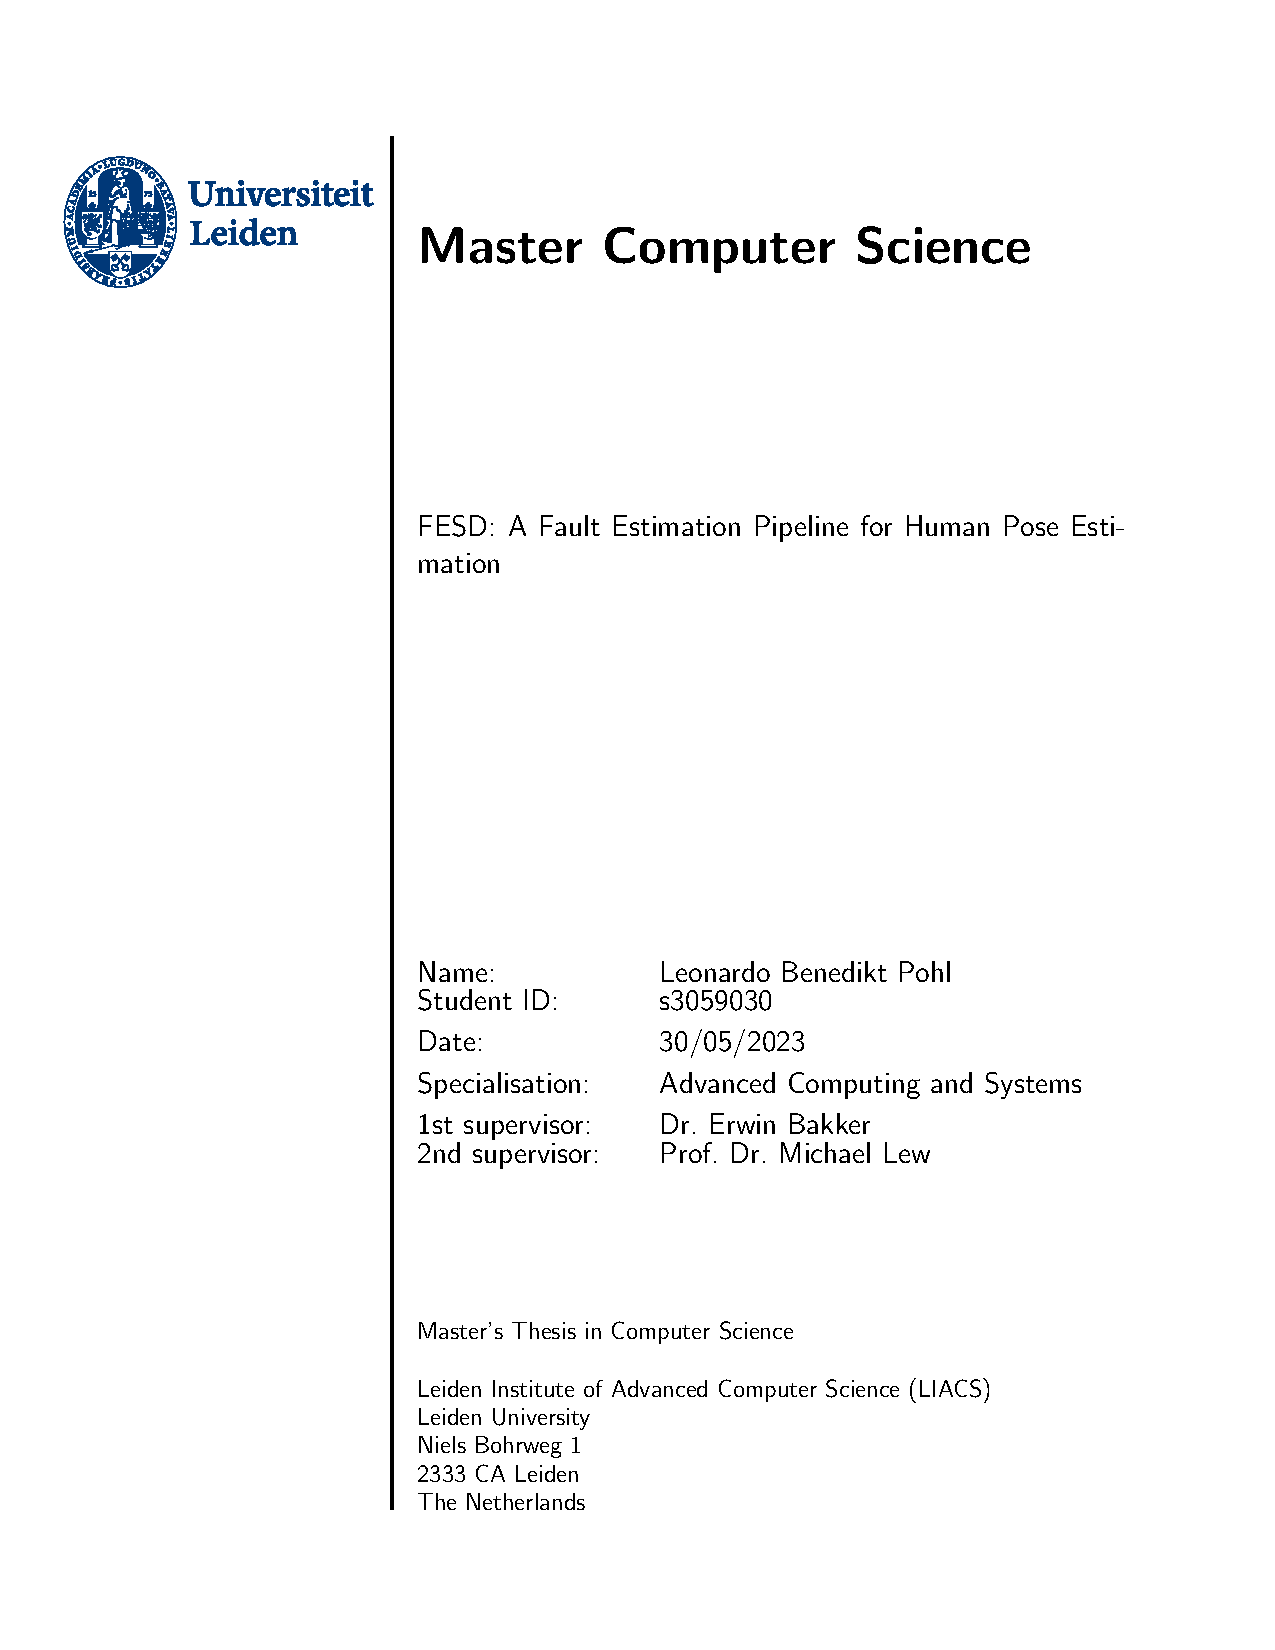
\includepdf[pages=1]{title_page.pdf}
\setlength{\voffset}{\originalVOffset}
\setlength{\hoffset}{\originalHOffset}

\clearpage

\begin{abstract}
  Human pose estimation(HPE), or skeleton detection, has been a topic of research for many years. With the advancement of hardware, it has become viable to apply HPE in real-time applications such as games. However, HPE is a difficult task that is prone to errors or faults, especially in complicated situations, such as cramped environments. These errors might cause human-computer interaction to be hampered.

  The goal of this thesis is to (1) understand what causes the problems, and (2) to design exercises which deliberately cause common errors and (3) to capture them within a dataset and label the entries accordingly. Finally, (4) preliminary models are developed to detect the errors or faults caused by HPE using the dataset.

  In this work, a tool is developed that is capable of capturing and labelling multi-modal data, \textbf{F}ault \textbf{E}stimator for \textbf{S}keleton \textbf{D}etection \textbf{Data} processor (FESDData). Four different datasets are captured using four problem sets with varying granularity, ranging from body-wise fault estimation to joint-wise fault estimation. Using the captured dataset, FESDDataset, preliminary experiments were run. For the preliminary experiments multiple models were developed one model for each of the problem sets, which aim to detect if an error occurs at different levels, \textbf{F}ault \textbf{E}stimator for \textbf{S}keleton \textbf{D}etection \textbf{Model} (FESDModelv1 and FESDModelv2). While version one of the models uses custom feature extraction the second version uses transfer learning using EfficientNetv2.

  In this thesis, common error sources that occur during HPE are found. Based on these error sources, exercises are derived which are captured in the FESDDataset using the dataset collection tool FESDData. The joints of the poses are then labelled based on the errors that occur. I abstract the data to form four different problem sets. For each of the problem sets, two models FESDModelv1 and FESDModelv2, are trained. The results of the preliminary experiments showed that FESDModelv1 outperforms FESDModelv2. Furthermore, from the four defined problem sets, both versions of the model perform best on the half-body problem set. In particular, the best results were achieved when considering the lower body. However, with further research and data FESDModelv1 and FESDModelv2 could be improved.

In conclusion, the preliminary models showed that the data captured by FESDData can successfully be used to create a model for fault estimation for skeleton detection.

\end{abstract}
